%% LyX 2.3.4.2 created this file.  For more info, see http://www.lyx.org/.
%% Do not edit unless you really know what you are doing.
\documentclass[english,dvipsnames,aspectratio=169,handout]{beamer}
\usepackage{mathptmx}
\usepackage{eulervm}
\usepackage[T1]{fontenc}
\usepackage[latin9]{inputenc}
\usepackage{babel}
\usepackage{amstext}
\usepackage{amssymb}
\usepackage{graphicx}
\usepackage{ifthen}
\usepackage{xcolor}
\usepackage{xspace}
\usepackage{tikz}
\usetikzlibrary{tikzmark}
\usetikzlibrary{calc}
\usepackage{pgfplots}
%\pgfplotsset{compat=1.17}
\usepackage{booktabs}
\usepackage{xpatch}
\usepackage{multirow}
\usepackage{colortbl}
\usepackage{pgfpages}

\newcommand{\commenteq}[1]{{\color{brown}#1}}
\newcommand{\alarm}[1]{{\color{red}#1}}



\xpatchcmd{\itemize}
  {\def\makelabel}
  {\ifnum\@itemdepth=1\relax
     \setlength\itemsep{2ex}% separation for first level
   \else
     \ifnum\@itemdepth=2\relax
       \setlength\itemsep{1ex}% separation for second level
     \else
       \ifnum\@itemdepth=3\relax
         \setlength\itemsep{0.5ex}% separation for third level
   \fi\fi\fi\def\makelabel
  }
 {}
 {}

\ifx\hypersetup\undefined
  \AtBeginDocument{%
    \hypersetup{unicode=true,pdfusetitle,
 bookmarks=true,bookmarksnumbered=false,bookmarksopen=false,
 breaklinks=false,pdfborder={0 0 0},pdfborderstyle={},backref=false,colorlinks=true,
 allcolors=NYUPurple,urlcolor=LightPurple}
  }
\else
  \hypersetup{unicode=true,pdfusetitle,
 bookmarks=true,bookmarksnumbered=false,bookmarksopen=false,
 breaklinks=false,pdfborder={0 0 0},pdfborderstyle={},backref=false,colorlinks=true,
 allcolors=NYUPurple,urlcolor=LightPurple}
\fi

\makeatletter

%%%%%%%%%%%%%%%%%%%%%%%%%%%%%% LyX specific LaTeX commands.
%% Because html converters don't know tabularnewline
\providecommand{\tabularnewline}{\\}

%%%%%%%%%%%%%%%%%%%%%%%%%%%%%% Textclass specific LaTeX commands.
% this default might be overridden by plain title style
\newcommand\makebeamertitle{\frame{\maketitle}}%
% (ERT) argument for the TOC
\AtBeginDocument{%
  \let\origtableofcontents=\tableofcontents
  \def\tableofcontents{\@ifnextchar[{\origtableofcontents}{\gobbletableofcontents}}
  \def\gobbletableofcontents#1{\origtableofcontents}
}

%%%%%%%%%%%%%%%%%%%%%%%%%%%%%% User specified LaTeX commands.
\usetheme{CambridgeUS} 
\beamertemplatenavigationsymbolsempty


% Set Color ==============================
\definecolor{NYUPurple}{RGB}{87,6,140}
\definecolor{LightPurple}{RGB}{165,11,255}


\setbeamercolor{title}{fg=NYUPurple}
\setbeamercolor{frametitle}{fg=NYUPurple}

\setbeamercolor{background canvas}{fg=NYUPurple, bg=white}
\setbeamercolor{background}{fg=black, bg=NYUPurple}

\setbeamercolor{palette primary}{fg=black, bg=gray!30!white}
\setbeamercolor{palette secondary}{fg=black, bg=gray!20!white}
\setbeamercolor{palette tertiary}{fg=gray!20!white, bg=NYUPurple}

\setbeamertemplate{headline}{}
\setbeamerfont{itemize/enumerate body}{}
\setbeamerfont{itemize/enumerate subbody}{size=\normalsize}

\setbeamercolor{parttitle}{fg=NYUPurple}
\setbeamercolor{sectiontitle}{fg=NYUPurple}
\setbeamercolor{sectionname}{fg=NYUPurple}
\setbeamercolor{section page}{fg=NYUPurple}
%\setbeamercolor{description item}{fg=NYUPurple}
%\setbeamercolor{block title}{fg=NYUPurple}

\setbeamertemplate{blocks}[rounded][shadow=false]
\setbeamercolor{block body}{bg=normal text.bg!90!NYUPurple}
\setbeamercolor{block title}{bg=NYUPurple!30, fg=NYUPurple}



\AtBeginSection[]{
  \begin{frame}
  \vfill
  \centering
\setbeamercolor{section title}{fg=NYUPurple}
 \begin{beamercolorbox}[sep=8pt,center,shadow=true,rounded=true]{title}
    \usebeamerfont{title}\usebeamercolor[fg]{title}\insertsectionhead\par%
  \end{beamercolorbox}
  \vfill
  \end{frame}
}

\makeatother

\setlength{\parskip}{\medskipamount} 

\input ../macros

\begin{document}
\input ../rosenberg-macros

%\setbeameroption{show notes on second screen}

\title[DS-GA 1003]{Forward Stagewise Additive Modeling}
\author{He He}
\date{April 13, 2021}
\institute{CDS, NYU}

\makebeamertitle
\mode<article>{Just in article version}

\begin{frame}
{Today's lecture}
\begin{itemize}
\item Another way to get non-linear models in a linear form---adaptive basis function models.
\item A general algorithm for greedy function approximation---gradient boosting machine.
\end{itemize}
\note[item]{We've learned kernel methods which gives you a non-linear classifier in a linear form. Today we are going to learn another method called ``adaptive basis function models''.
}
\note[item]{And we are going to learn a general algorithm for learning these basis functions, which give rise to a family of boosting algorithms, including Adaboost we saw last time.}
\end{frame}

\section{Motivation}
\begin{frame}
{Recap: Adaboost}
\begin{center}
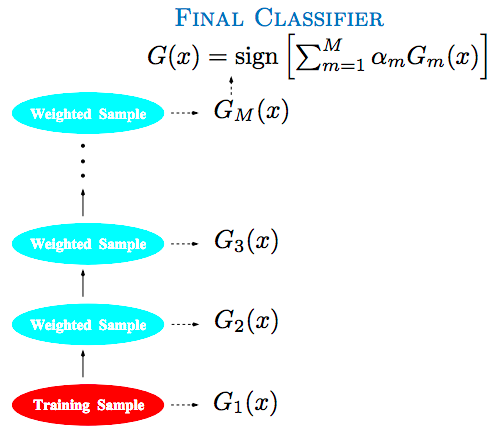
\includegraphics[height=0.7\textheight]{figures/adaboostSchematic}
\par\end{center}
\let\thefootnote\relax\footnotetext{\tiny{From ESL Figure 10.1}}
\note[item]{Recall the Adaboost algorithm we talked about last time. We want to learn a sequence of base classifiers; each of them minimizes weighted zero-one error, where the weights are higher on previously misclassified examples. It's like when you study for an exam, you go over all practice questions; then you look at the answers. The next time you spend more time on questions you go wrong. In the end you would grasp everything.}
\note[item]{Our final classifier is a weighted combination the base classifiers. The weights on good classifiers are higher, where ``good'' is measured by weighted zero-one error.}
\note[item]{Last time we went over a greedy algorithm for obtaining the base classifiers and the weights. Let's review the Adaboost algorithm.}
\end{frame}

\begin{frame}{AdaBoost: Algorithm}

Given training set $\cd=\left\{ \left(x_{1},y_{1}\right),\ldots,\left(x_{n},y_{n}\right)\right\} $.
\begin{enumerate}
\item Initialize observation weights $w_{i}=1$, $i=1,2,\ldots,n$.

\item For $m=1$ to $M$:
\begin{enumerate}
\item Base learner fits weighted training data and returns $G_{m}(x)$

\item Compute \emph{weighted empirical 0-1 risk}:
\[
\mbox{err}_{m}=\frac{1}{W}\sum_{i=1}^{n}w_{i}\ind{y_{i}\neq G_{m}(x_{i})}\quad\text{where }W=\sum_{i=1}^{n}w_{i}.
\]

\item Compute  \emph{classifier weight}: $\alpha_{m}=\ln\left(\frac{1-\text{err}_{m}}{\text{err}_{m}}\right)$.

\item Update \emph{example weight}: $w_{i}\gets w_{i}\cdot\exp\left[\alpha_{m}\ind{y_{i}\neq G_{m}(x_{i})}\right]$
\end{enumerate}
\item Return \emph{voted classifier}: $G(x)=\sign\left[\sum_{m=1}^{M}\alpha_{m}G_{m}(x)\right]$.
\onslide<+->{\hspace{2em}{\color{red}Why not learn $G(x)$ directly?}}
\end{enumerate}
\note[item]{But why does this algorithm work? Does it actually gives us a good classifier in our hypothesis space? Let's work backwards. Since $G(x)$ is the final model we want, why don't we learn it directly? This is actually a special case of additive basis function models.}
\end{frame}

\begin{frame}{Nonlinear Regression}
\begin{itemize}
\item How do we fit the following data?
\begin{figure}
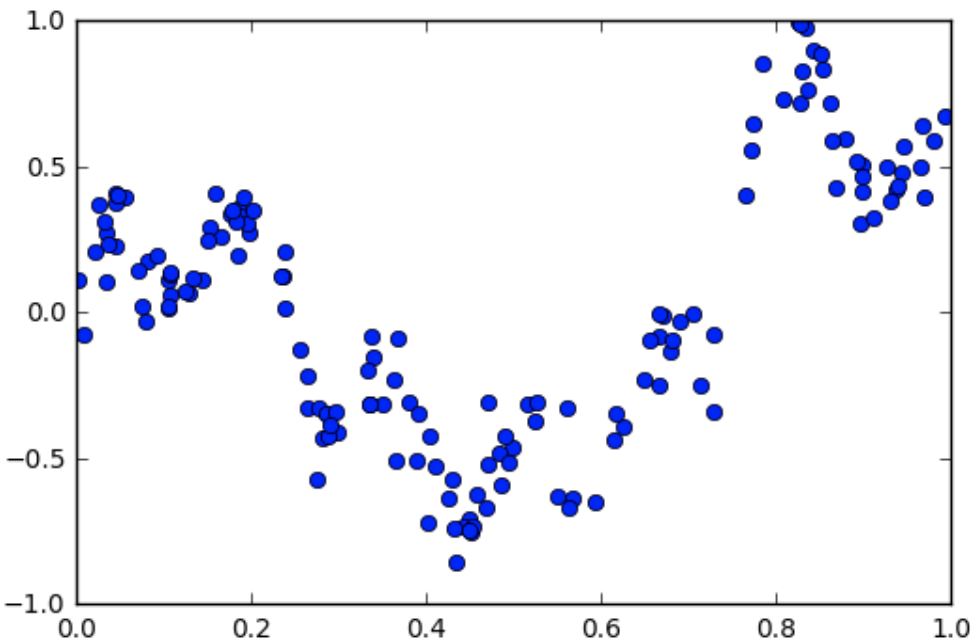
\includegraphics[height=0.6\textheight]{figures/nonlinear-regression-data}
\end{figure}
\end{itemize}
\note[item]{To motivate adaptive basis models, let's consider this nonlinear regression problem. Given the following data, what model would you use?}
\note[item]{We can create non-linear features.}
\end{frame}
%
\begin{frame}{Linear Model with Basis Functions}
\begin{itemize}[<+->]
\item Fit a linear combination of transformations of the input:
\[
f(x)=\sum_{m=1}^{M}v_{m}h_{m}(x),
\]
where $h_m$'s are called \textbf{basis functions} (or feature functions in ML):
\[
h_{1},\ldots,h_{M}:\cx\to\reals
\]
\item Example: polynomial regression where $h_m(x) = x^m$.
\item Can we use this model for classification?
\note[item]{$f(x)$ can be transformed to a probability (\eg similar to GLM), or used as a score function (\eg margin-based classification and ranking).}
\item Can fit this using standard methods for linear models (e.g. least
squares, lasso, ridge, etc.)
\begin{itemize}
\item \emph{Note that $h_m$'s are fixed and known}, \ie chosen ahead of time.
\end{itemize}
\end{itemize}
\note[item]{The key idea here is to use a family of functions or transformations that can be applied to $x$, which are called basis functions.}
\note[item]{The basis functions can be non-linear in $x$. Can you think of some examples? Polynomials, piecewise constant functions.}
\note[item]{We can use it for classification by another function to transform the results to a probability or a class, \eg sgn as in Adaboost.}
\note[item]{All inference methods we've learned for linear models can be applied here. Why? It's important to note that $h_m$ are fixed, thus they can be simply considered as another feature.}
\end{frame}
%
\begin{frame}{Adaptive Basis Function Model}
\begin{itemize}[<+->]
\item What if we want to learn the basis functions? (hence \emph{adaptive})

\item {Base hypothesis space} $\ch$ consisting of functions $h:\cx\to\reals$.

\item<.-> An \textbf{adaptive basis function expansion }over $\ch$ is
an ensemble model:
\begin{align}
f(x)=\sum_{m=1}^{M}v_{m}h_{m}(x),
\end{align}
where $v_{m}\in\reals$ and $h_{m}\in\ch$.

\item Combined hypothesis space:
\[
\cf_{M}=\left\{ \sum_{m=1}^{M}v_{m}h_{m}(x)\mid v_{m}\in\reals,\:h_{m}\in\ch,\:m=1,\ldots,M\right\} 
\]
\item<.-> What are the learnable?
\end{itemize}
\note[item]{But in Adaboost we don't know the base classifier beforehand. How to learn them?}
\note[item]{Let's formalize the problem a bit. The basis functions belong to the base hypothesis space, and our predictor is a linear combination of the basis functions, just as every vector in a vector space can be represented by a linear combination of the basis vectors.}
\note[item]{Both the weights $v_m$ and  the basis functions $h_m$ are learned, as in Adaboost.}
\end{frame}
%
%\begin{frame}{Adaptive Basis Function Model}
%\begin{itemize}
%\item \textbf{Base hypothesis space}: $\ch$ of \textbf{real-valued functions} 
%\item \textbf{Combined hypothesis space:} $\cf_{M}$:
%\[
%\cf_{M}=\left\{ \sum_{m=1}^{M}v_{m}h_{m}(x)\mid v_{m}\in\reals,\:h_{m}\in\ch,\:m=1,\ldots,M\right\} 
%\]
%
%\pause{}
%\item Suppose we're given some data $\cd=\left((x_{1},y_{1}),\ldots,(x_{n},y_{n})\right)$.
%
%\pause{}
%\item Learning is choosing $v_{1},\ldots,v_{M}\in\reals$ and $h_{1},\ldots,h_{M}\in\ch$
%to fit $\cd$.
%\end{itemize}
%\end{frame}

%\begin{frame}{Not Limited to Regression}
%\begin{itemize}
%\item Linear combination of basis functions:
%\[
%f(x)=\sum_{m=1}^{M}v_{m}g_{m}(x)
%\]
%\item $f(x)$ is a number \textemdash{} for regression, it's exactly what
%we're looking for.
%
%\pause{}
%\item Otherwise, $f(x)$ is often called a \textbf{score} function.
%\item It can be 
%\begin{itemize}
%\item thresholded to get a classification
%\item transformed to get a probability
%\item transformed to get a parameter of a probability distribution (e.g.
%Poisson regression)
%\item used for ranking search results
%\end{itemize}
%\end{itemize}
%\end{frame}
%

%
\begin{frame}{Empirical Risk Minimization}
\begin{itemize}[<+->]
\item What's our learning objective? 
\[
\hat{f}=\argmin_{f\in\cf_{M}}\frac{1}{n}\sum_{i=1}^{n}\ell\left(y_{i},f(x_{i})\right),
\]
for some {loss function} $\ell$. 

\item Write ERM objective function as
\[
J(v_{1},\ldots,v_{M},h_{1},\ldots,h_{M})=\frac{1}{n}\sum_{i=1}^{n}\ell\left(y_{i},\sum_{m=1}^{M}v_{m}h_{m}(x)\right).
\]

\item How to optimize $J$? i.e. how to learn?
\end{itemize}
\note[item]{So the main question left is how to optimize $J$. Adaboost uses a greedy algorithm. But can we directly optimize all parameters?}
\end{frame}
%
\begin{frame}{Gradient-Based Methods}
\begin{itemize}[<+->]
\item \texttt{Suppose} our base hypothesis space is parameterized by $\Theta=\reals^{b}$:
\[
J(v_{1},\ldots,v_{M},{\color{blue}\theta_{1},\ldots,\theta_{M}})=\frac{1}{n}\sum_{i=1}^{n}\ell\left(y_{i},\sum_{m=1}^{M}v_{m}h(x;{\color{blue}\theta_{m}})\right).
\]

\item Can we optimize it with SGD?
\begin{itemize}
\item Can we differentiate $J$ w.r.t. $v_{m}$'s and $\theta_{m}$'s?
\end{itemize}

\item For {some} hypothesis spaces and typical loss functions, yes!
\begin{itemize}[<.->]
\item Neural networks fall into this category! ($h_{1},\ldots,h_{M}$ are
neurons of last hidden layer.)
\end{itemize}
\end{itemize}
\note[item]{Note that $h$ doesn't have to be a parametric model; it can be non-parametric, \eg decision trees.}
\note[item]{Running SGD requires the objective to be differentiable w.r.t. the parameters, \eg neural networks.}
\end{frame}
%
\begin{frame}{What if Gradient Based Methods Don't Apply?}
\begin{simpleblock}
{{What if base hypothesis space $\ch$ consists of decision trees?}}
\begin{itemize}[<2->]
\item Can we even parameterize trees with $\Theta=\reals^{b}$?
\item Even if we could, predictions would not change continuously w.r.t. $\theta\in\Theta$, so certainly not differentiable.
\end{itemize}
\end{simpleblock}
\note[item]{First of all, we cannot really parametrize decision trees as the number of parameters depends on the tree structure. But even if we fix the tree structure, in which case the parameters are the splitting feature values, we still cannot run SGD as the function is piecewise-constant.}

\begin{simpleblock}
{\onslide<3->{What about a greedy algorithm similar to Adaboost?}}
\begin{itemize}[<4->]
\item Applies to non-parametric or non-differentiable basis functions.
\item But is it optimizing our objective using some loss function?
\end{itemize}
\end{simpleblock}
\note[item]{Adaboost gives us a model in the form of an adaptive basis function model. But what the objective function it is optimizing?}

\onslide<5->{
\begin{simpleblock}
{Today we'll discuss \textbf{gradient boosting}.}
\begin{itemize}
\item Gradient descent in the \emph{function space}.
\item It applies whenever 
\begin{itemize}
\item our loss function is {[}sub{]}differentiable w.r.t. training predictions
$f(x_{i})$, and
\item we can do regression with the base hypothesis space $\ch$.
\end{itemize}
\end{itemize}
\end{simpleblock}
}

\note[item]{Using gradient boosting, we can directly optimize the basis functions in the function space.}
\note[item]{We will show that Adaboost is just a special case of gradient boosting using the exponential loss.}
\note[item]{This algorithm is very general, it only requires...}
\end{frame}
%

\begin{frame}
{History}
\begin{table}
\begin{tabular}{rp{8cm}}
Kearns, Valiant (1989): & Can weak learners (\eg $51\%$ accuracy) be transformed to strong learners (\eg $99.9\%$ accuracy)?\pause \\
Schapire (1990) \& Freund (1995): & Yes, weak learners can be iteratively improved to a strong learner.\pause \\
Freund, Schapire (1996): & And here is a practical algorithm---Adaboost.\pause \\
Breiman (1996 \& 1998): & Yes, it works! Boosting is the best off-the-shelf classifier in the world.\pause \\
\multicolumn{2}{c}{(Attempts to explain why Adaboost works and improvements)}\pause\\
Friedman, Hastie, Tibshirani (2000): & Actually, boosting fits an additive model.\pause \\
Friedman (2001): & Furthermore, it can be considered as gradient descent in the function space.
\end{tabular}
\end{table}
\note[item]{The idea of boosting started from a theoretical question: can we transform weak learners that are merely better than chance to arbitrarily strong learners?}
\note[item]{Schapir and Freund first gave an affirmative answer. However their boosting algorithm at that time was mainly constructed for theoretical proofs. In 1996, Adaboost was born.}
\note[item]{There is a lot of excitement in the ML community around it. In particular, Leo Breiman, who contributed many ideas we learned last week including CART, bagging, and random forest, said that...}
\note[item]{Then there are many attempts to explain why it works, variations and improvements. Finally, in 2000, FHT (the authors of one of our reference books, ESL) gave a statistical view of boosting. It in fact fits an additive model.}
\note[item]{Friedman further elaborates the idea using gradient descent in the function space, which we will learn about today.}
\end{frame}

%\begin{frame}{Overview}
%\begin{itemize}
%\item Forward stagewise additive modeling (FSAM)
%\begin{itemize}
%\item example: $L^{2}$ Boosting 
%\item example: exponential loss gives AdaBoost
%\item Not clear how to do it with many other losses, including logistic
%loss
%\end{itemize}
%\item Gradient Boosting
%\begin{itemize}
%\item example: logistic loss gives BinomialBoost
%\end{itemize}
%\item Variations on Gradient Boosting
%\begin{itemize}
%\item step size selection
%\item stochastic row/column selection
%\item Newton step direction
%\item XGBoost
%\end{itemize}
%\end{itemize}
%\end{frame}

\section{Forward Stagewise Additive Modeling }
\begin{frame}{Forward Stagewise Additive Modeling (FSAM)}
\begin{description}
\item[Goal] fit model $f(x) = \sum_{m=1}^M v_mh_m(x)$ given some loss function.
\item[Approach]
{Greedily} fit one function at a time without adjusting previous functions, hence ``forward stagewise''.
\end{description}

\begin{itemize}[<+->]
\item After $m-1$ stages, we have
\[
f_{m-1}=\sum_{i=1}^{m-1}v_{i}h_{i}.
\]
 
\item In $m$'th round, we want to find 
$h_{m}\in\ch$ (i.e. a basis function) and
$v_{m}>0$ 
such that 
\[
f_{m}=\underbrace{f_{m-1}}_{\text{fixed}}+v_{m}h_{m}
\]
improves objective function value by as much as possible.
\end{itemize}
\note[item]{At the $m$'th stage, we would have trained $m-1$ classifiers, so the current classifier is a combination of the previous $m-1$ classifiers.}
\note[item]{And we will fit the next basis function $h_m$ and $v_m$ to improve the objective function value as much as possible. Here we consider $f_{m-1}$ fixed and known.
Note that in each round, we are only doing local improvement w.r.t. the $m$'th basis function.}
\end{frame}
%
\begin{frame}{Forward Stagewise Additive Modeling for ERM}
Let's plug in our objective function.
\begin{enumerate}
\item Initialize $f_{0}(x)=0$.
\item For $m=1$ to $M$:

\pause{}
\begin{enumerate}
\item Compute:
\[
\left(v_{m},h_{m}\right)=\argmin_{v\in\reals,h\in\ch}\frac{1}{n}\sum_{i=1}^{n}\ell\left(y_{i},f_{m-1}(x_{i})\underbrace{+v h(x_{i})}_{\text{new piece}}\right).
\]


\pause{}
\item Set $f_{m}=f_{m-1}+v_{m}h_m$.

\pause{}
\end{enumerate}
\item Return: $f_{M}$.
\end{enumerate}
\note[item]{We fit $M$ basis functions sequentially. In each round, we find the next basis function $h_m$ and its weight $v_m$ that minimizes the empirical risk.
And we add that to our current model $f$.}
\note[item]{In the end, we return a weighted sum of the $M$ basis functions.}
\note[item]{Next, we will show that Adaboost is FSAM with exponential loss.}
\end{frame}
%

\subsection{Example: AdaBoost}
\begin{frame}{Recap: margin-based classifier}
\begin{simpleblock}
{Binary classification}
\begin{itemize}
\item Outcome space $\cy=\left\{ -1,1\right\} $
\item Action space $\ca=\reals$ (model outoput)
\item Score function $f:\cx\to\ca$.
\item Margin for example $(x,y)$ is $m=yf(x)$. 
\begin{itemize}
\item $m>0\iff$ classification correct
\item Larger $m$ is better.
\end{itemize}
\item \think{Concept check}: What are margin-based loss functions we've seen?
\end{itemize}
\end{simpleblock}
\note[item]{Exponential loss is a margin-based loss function. Before talking about the exponential loss, let's first do a quick recap of margin-based classifier.}
\note[item]{Other margin-based loss: hinge loss, logistic loss in HW5.}
\end{frame}
%
%
\begin{frame}{Exponential Loss}
\begin{itemize}
\item Introduce the \textbf{exponential loss}: $\ell(y,f(x))=\exp\left(-\underbrace{yf(x)}_{\text{margin}}\right).$
\end{itemize}
\begin{center}
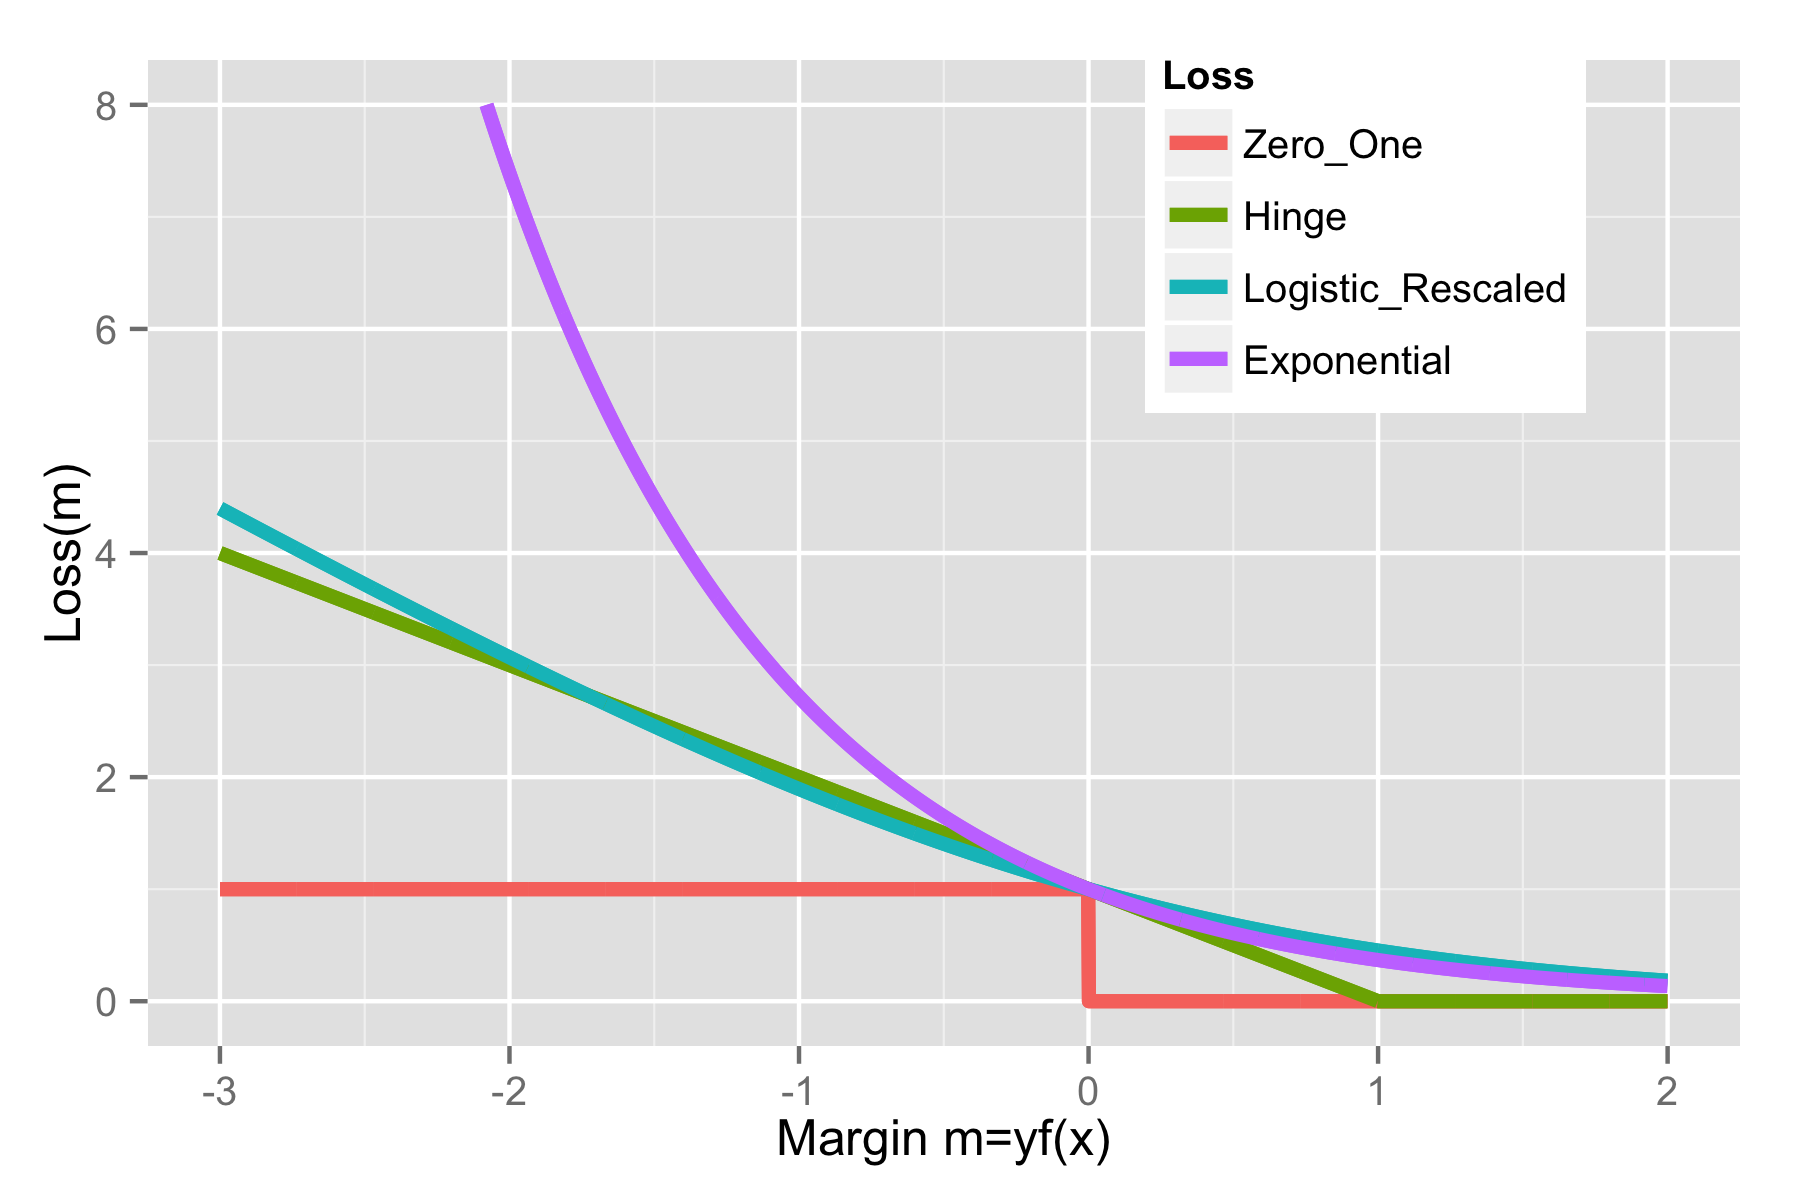
\includegraphics[height=0.65\textheight]{{figures/loss.Zero_One.Hinge.Logistic_Rescaled.Exponential}.png}
\par\end{center}
\note[item]{The exponential loss is just the exponential of negative margin. It is also a convex upperbound of the zero-one loss.}
\end{frame}
%
\begin{frame}{Forward Stagewise Additive Modeling with exponential loss}
Recall that we want to do FSAM with exponential loss.
\begin{enumerate}
\item Initialize $f_{0}(x)=0$.
\item For $m=1$ to $M$:
\begin{enumerate}
\item Compute:
\[
\left(v_{m},h_{m}\right)=\argmin_{v\in\reals,h\in\ch}\frac{1}{n}\sum_{i=1}^{n}{\color{blue}\ell_{\text{exp}}}\left(y_{i},f_{m-1}(x_{i})\underbrace{+v h(x_{i})}_{\text{new piece}}\right).
\]
\item Set $f_{m}=f_{m-1}+v_{m}h_m$.
\end{enumerate}
\item Return: $f_{M}$.
\end{enumerate}
\note[item]{Now let's plug in our loss function in FSAM.}
\end{frame}

\begin{frame}{FSAM with Exponential Loss: objective function}
\begin{itemize}
\item Base hypothesis: $\sH = \pc{h\colon \sX \rightarrow \pc{-1, 1}}$.
\item Objective function in the $m$'th round:
\pause
\begin{align}
J(v, h) &= \sum_{i=1}^n \exp\pb{
-y_i \p{ f_{m-1}(x_i) + vh(x_i) }
} \\
&= \sum_{i=1}^n w_i^m \exp\pb{ -y_ivh(x_i) } &&  \commenteq{w_i^m \eqdef \exp\pb{ -y_i f_{m-1}(x_i) } }\\
&= \sum_{i=1}^n w_i^m \pb{ \1\p{y_i=h(x_i)}e^{-v} + \1\p{y_i\neq h(x_i)}e^v } 
&& \commenteq{h(x_i) \in \pc{1, -1}} \\
&=  \sum_{i=1}^n w_i^m \pb{ (e^v-e^{-v})\1\p{y_i\neq h(x_i)} + e^{-v} }
&& \commenteq{\1\p{y_i=h(x_i)} = 1- \1\p{y_i\neq h(x_i)}}
\end{align}


\end{itemize}
\end{frame}
%
\begin{frame}{FSAM with Exponential Loss: basis function}
\begin{itemize}[<+->]
\item Objective function in the $m$'th round:
\begin{align}
J(v, h) &= \sum_{i=1}^n w_i^m \pb{ (e^v-e^{-v})\1\p{y_i\neq h(x_i)} + e^{-v} } .
\end{align}
\item If $v>0$, then
\begin{align}
\onslide<.->{
\argmin_{h\in\sH}J(v,h) &=
\argmin_{h\in\sH} \sum_{i=1}^n w_i^m \1\p{y_i\neq h(x_i)} \\
}
\onslide<+->{
h_m &= \argmin_{h\in\sH} \sum_{i=1}^n w_i^m \1\p{y_i\neq h(x_i)} \\
}
\onslide<+->{
&= \argmin_{h\in\sH} \frac{1}{\sum_{i=1}^n w_i^m} \sum_{i=1}^n w_i^m \1\p{y_i\neq h(x_i)}
&& \commenteq{\text{multiply by a positive constant}}
}
\end{align}
\onslide<+->{
\ie $h_m$ is the minimizer of the weighted zero-one loss.
}
\end{itemize}
\note[item]{Let's first find the optimal $h$, the last term does not depend on $h$ so it can be ignored for now. Do we want the indicator to be one or zero? It depends on the coefficient.}
\end{frame}

\begin{frame}{FSAM with Exponential Loss: classifier weights}
\begin{itemize}[<+->]
\item Define the weighted zero-one error:
\begin{align}
\text{err}_m = \frac{\sum_{i=1}^n w_i^m \1\p{y_i\neq h(x_i)}}{\sum_{i=1}^n w_i^m} .
\end{align}
\item \think{Exercise}: show that the optimal $v$ is:
\begin{align}
v_m = \frac{1}{2}\log\frac{1-\text{err}_m}{\text{err}_m}
\end{align}
\begin{itemize}
\item Same as the classifier weights in Adaboost (differ by a constant).
\item If $\text{err}_m < 0.5$ (better than chance), then $v_m > 0$.
\end{itemize}
\end{itemize}
\note[item]{Now let's fine the optimal weight $v$.}
\note[item]{To simplify notation, let's define $err_m$. Since $v$ is a real number, you can compute the gradient w.r.t. $v$ and set it to zero.}
\note[item]{Remember that we assumed $v>0$. Is it true for optimal $v$?}
\end{frame}

\begin{frame}
{FSAM with Exponential Loss: example weights}
\begin{itemize}
\item Weights in the next round:
\begin{align}
w_i^{m+1} &\eqdef \exp\pb{ -y_i f_m(x_i) } \\
\onslide<2->{
&= w_i^m \exp\pb{ -y_i v_m h_m(x_i) } 
\quad\quad\quad \commenteq{f_m(x_i) = f_{m-1}(x_i) + v_mh_m(x_i)} \\
&= w_i^m \exp\pb{ -v_m\1\p{y_i = h_m(x_i)} + v_m\1\p{y_i \neq h_m(x_i)} } \\
&= w_i^m \exp\pb{ 2v_m\1\p{y_i \neq h_m(x_i)} } \underbrace{\exp^{-v_m}}_{\text{scaler}}
}
\end{align}
\item<3-> The constant scaler will cancel out during normalization.
\item<4-> $2v_m = \alpha_m$ in Adaboost.
\end{itemize}
\note[item]{So far we have shown that FSAM with exponential loss also fits base classifiers using the weighted zero-one loss, and classifier weights is the same as Adaboost. But what about the example weights?}
\note[item]{The example weights are updated in the same way too! If an example is misclassified, we increase its weight same as in Adaboost.}
\note[item]{Now we have derived Adaboost using FSAM with exponential loss.}
\end{frame}

\begin{frame}{Why Exponential Loss}
\begin{itemize}[<+->]
\item $\ell_{\text{exp}}(y, f(x)) = \exp(-yf(x))$.
\item \think{Exercise}: show that the optimal estimate is
\begin{align}
f^*(x) = \frac{1}{2}\log\frac{p(y=1\mid x)}{p(y=0\mid x)} .
\end{align}
\item How is it different from other losses?
\begin{center}
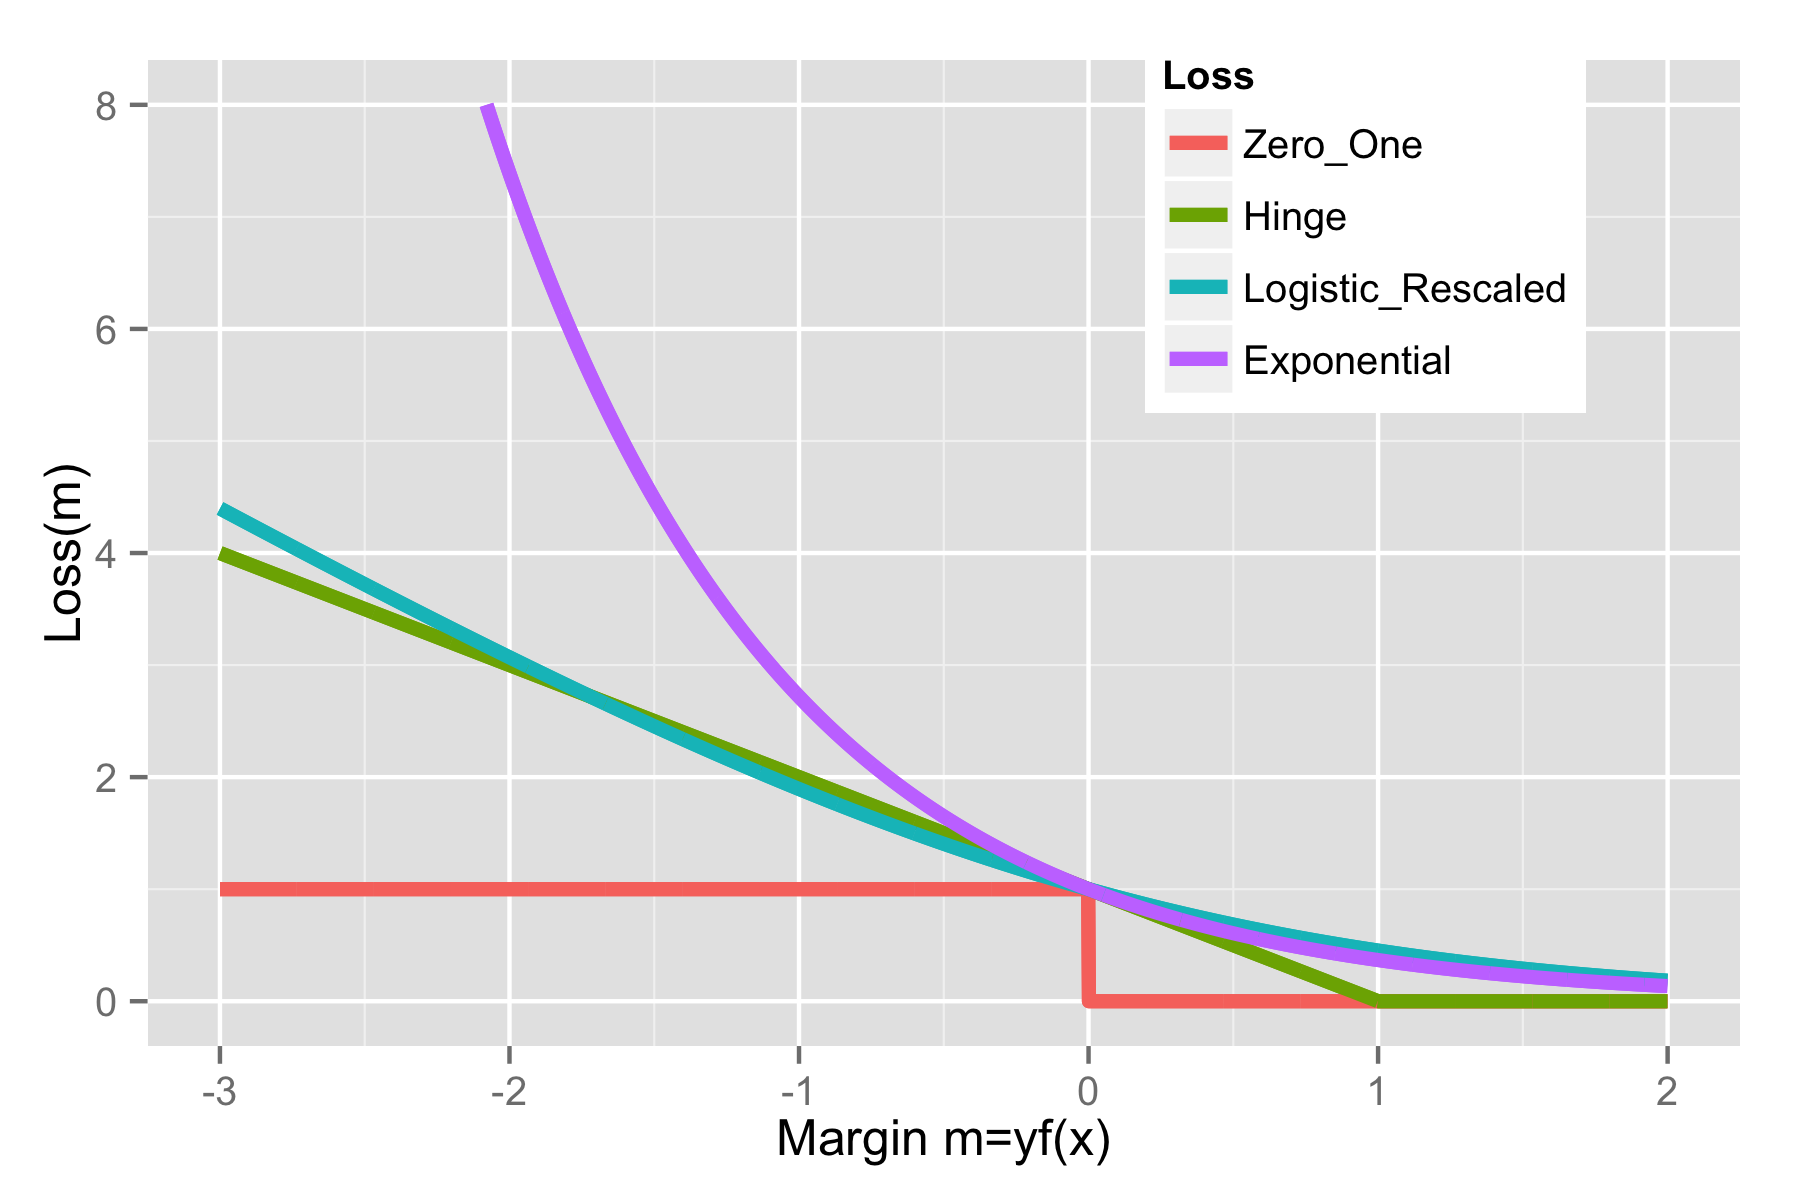
\includegraphics[height=0.45\textheight]{{figures/loss.Zero_One.Hinge.Logistic_Rescaled.Exponential}.png}
\end{center}
\end{itemize}
\note[item]{Adaboost was not initially designed to minimize exponential loss. It's only discovered 5 years after its invention. In the FSAM context, the main motivation for using exponential loss is computational: it leads to a simple optimization algorithm through example reweighting. But let's think about why this loss function makes sense from the statistical learning perspective.}
\note[item]{We can show that the optimal $f(x)$ is estimating one-half of the log odds. This justifies using the sign of it the make map the score to -1 and 1, \ie optimal under bayes decision rule.}
\note[item]{We have seen in logistic regression that its optimal estimate is also the log odds. So they will given the same model if there's infinite data. But in the finite-sample case, their behavior will be different.}
\note[item]{It puts more penalty on wrong predictions.}
\end{frame}
%
\begin{frame}{AdaBoost / Exponential Loss: Robustness Issues}
\begin{itemize}
\item Exponential loss puts a high penalty on misclassified examples.
\pause
\begin{itemize}
\item $\implies$ not robust to outliers / noise.
\end{itemize}
\item Empirically, AdaBoost has degraded performance in situations with 
\begin{itemize}
\item high Bayes error rate (intrinsic randomness in the label)
\end{itemize}
\pause
\item Logistic/Log loss performs better in settings with high Bayes error.
%\begin{itemize}
\item Exponential loss has some computational advantages over log loss though.
%\item FSAM + log loss $\implies$ LogitBoost
%\end{itemize}
\end{itemize}
\note[item]{Why is it bad? It means that the model will try very hard on a few misclassified examples.}
\end{frame}
%
\begin{frame}{Review}
We've seen
\begin{itemize}
\item Use basis function to obtain \emph{nonlinear} models: $f(x) = \sum_{i=1}^M v_m h_m(x)$ with known $h_m$'s.
\item \emph{Adaptive} basis function models: $f(x) = \sum_{i=1}^M v_m h_m(x)$ with unknown $h_m$'s.
\item Forward stagewise additive modeling: greedily fit $h_m$'s to minimize the average loss.
\end{itemize}
\pause
But,
\begin{itemize}
\item We only know how to do FSAM for certain loss functions.
\item Need to derive new algorithms for different loss functions.
\end{itemize}

Next, how to do FSAM in general.
\note[item]{Let's recap now. We started with the nonlinear regression problem. One way to obtain nonlinear classifier in the linear form is through basis functions, which compute a nonlinear transformation of $x$.}
\note[item]{If $h_m$ is known, that's easy---the problem is reduced to linear models. But what if we want to learn $h_m$'s?}
\note[item]{Last week we saw how to use the iterative Adaboost algorithm to find these base classifiers or basis functions. Today we saw that it's a special case of FSAM using exponential loss.}
\note[item]{In the FSAM framework, it is easy to plug in new loss functions.}
\end{frame}
%


\end{document}
